\problemname{Brädspelet}
Ann-Charlotte och Berit har uppfunnit ett eget brädspel. Spelet spelas med ett
bräde av storlek $N \times M$ dm samt en motorsåg, och är till för två spelare.
Spelarna turas om att göra drag tills någon av dem inte har något giltigt drag
längre, och denna spelaren förlorar. Ett drag går till på följande sätt:

Spelaren som är på tur väljer en horisontell eller vertikal linje och delar
brädet i två icke-tomma delar. Detta får dock endast göras vid heltalskoordinater (så att
dimensionerna av de två delarna alltid är heltal). Motspelaren väljer sedan en av
delarna, och spelet fortsätter med den medan den andra delen kastas. Eftersom
dimensionerna alltid måste vara heltal så är det alltid den som är på tur att
dela när brädet har storlek $1 \times 1$ som förlorar.

Givet storleken på det ursprungliga brädet, och det faktum att Ann-Charlotte
alltid börjar, kan du avgöra vem som vinner om de båda spelar optimalt?

\begin{figure}[ht!]
\centering
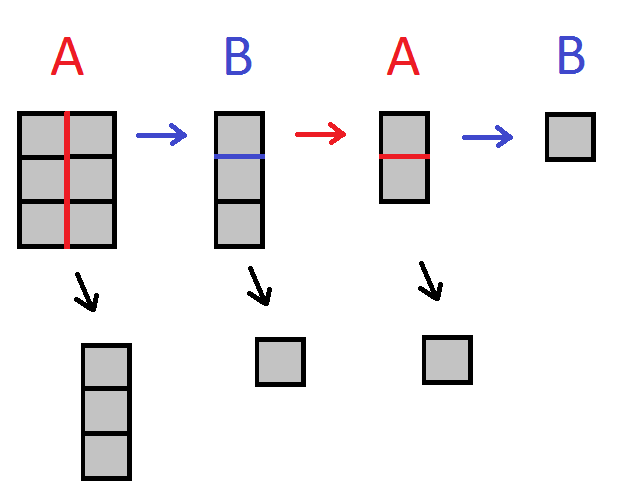
\includegraphics[width=0.7\textwidth]{bradspelet.png}
\caption{En illustration av det första exemplet.}
\label{overflow}
\end{figure}

\section*{Indata}
Indata består av en rad med de två talen $N$ och $M$ ($1 \le N,M \le 100$).

\section*{Utdata}

En rad med strängen "\texttt{A}" om Ann-Charlotte vinner och "\texttt{B}" om
Berit vinner, givet att de båda spelar optimalt. Mer precist, om Ann-Charlotte
kan vinna oavsett hur Berit spelar så ska du skriva "\texttt{A}", annars ska du
skriva "\texttt{B}".

\section*{Poängsättning}
Din lösning kommer att testas på en antal testfallsgrupper. För att få poäng för en grupp så måste du klara alla testfall i gruppen.

\noindent
\begin{tabular}{| l | l | l |}
	\hline
	Grupp & Poängvärde & Gränser\\ \hline
 $1$    & $20$        & $N, M \le 10$ \\ \hline
 $2$    & $80$        & Inga ytterligare begränsningar. \\ \hline
\end{tabular}


\section*{Förklaring av exempelfall 1}
I det första exemplet så vinner $A$ genom att dela brädet i två delar av storlek
$1 \times 3$. Oavsett hur $B$ sedan gör så får $A$ nästa gång välja mellan
delar av storlek $1 \times 2$ och $1 \times 1$. Rätt strategi är att välja $1
\times 2$ (det andra leder direkt till en förlust). $B$ tvingas sedan att välja
mellan två delar av storlek $1 \times 1$, som båda innebär förlust.
